\documentclass{article}
\usepackage[utf8]{inputenc}
\usepackage[spanish]{babel}
\usepackage{listings}
\usepackage{graphicx}
\graphicspath{ {images/} }
\usepackage{cite}

\begin{document}

\begin{titlepage}
    \begin{center}
        \vspace*{1cm}
            
        \Huge
        \textbf{Taller- Nociones de la memoria del computador}
            
        \vspace{0.5cm}
        \LARGE
        
            
        \vspace{1.5cm}
            
        \textbf{Ana Cristina Henao Guerra}\\
        \textbf{cc. 103767030}
            
        
        \vspace*{3cm}
        \large{profesor: Augusto Enrique Salazar Jimenez}
        \vfill
            
        \vspace{0.8cm}
            
        \Large
        Despartamento de Ingeniería Electrónica y Telecomunicaciones\\
        Universidad de Antioquia\\
        Medellín\\
        Septiembre de 2020
            
    \end{center}
\end{titlepage}

\tableofcontents
\newpage
\section{Sección introductoria}\label{intro}
Como es bien conocido, un computador está conformado por software y hardware, siendo el software, los componentes internos que hacen funcionar el computador (programas que componen el sistema interno), y el hardware son los elementos tangibles que permiten el acercamiento máquina-usuario, lo que a grandes rasgos nos indica, que la memoria de un computador forma parte del software. Se denomina memoria a aquel circuito que permite almacenar la información que más adelante será retomada para su uso, lo que muestra que la memoria son sistemas de almacenamiento y pueden ser de diferentes tipos, entre ellas disco duro, memoria RAM, memoria virtual, entre otras; La  gran diferencia se encuentra en la rapidez que manejan, dependiendo del tamaño y del tipo de memoria, algo importante para tener en cuenta, es que la memoria RAM es la que se encarga de mantener los programas abiertos y funcionando.
En la actualidad, las memorias de los computadores, han ido evolucionando para proporcionar mejor calidad y rapidez en la realización del trabajo en un computador.\\

Se debe tener presente al obtener un computador, la capacidad de memoria RAM, ya que de esta depende la eficiencia en la ejecucion de los trabajos en el equipo.

\subsection{Citación}
Documento basado en artículo: Como funciona la memoria de una computadora \textbf{Augusto Salazar} \cite{Salazar}.
El comienzo: El chip \textbf{página web}
\cite{website}
libro: Organizacion y arquitectura de computadores \textbf{William Stalling} \cite{Stalling}
Documento: Arquitectura de las computadoras-Memoria. Basadas en las Notas de Teórico Versión 1.0 del \textbf{Dpto. de Arquitectura-InCo-FIng}\cite{document}

\section{Sección de contenido} \label{contenido}
Dando solución a las siguientes preguntas definidas previamente en el taller, y con base en la lectura propuesta por el profesor Augusto Salazar:\\

%
1. Defina que es la memoria del computador.\\
2.Mencione los tipos de memoria que conoce y haga una pequeña descripción de cada tipo.\\
3. Describa la manera como se gestiona la memoria en un computador.\\
4. ¿Que hace que una memoria sea más rápida que otra? ¿Por qué esto es importante?\\


\subsection{Defina que es la memoria del computador}
%
La memoria del computador, es un dispositivo donde durante un tiempo, se almacena toda la información (binaria, denominada 'palabras') con la que posteriormente hacen uso los demás dispositivos del computador, como son los microprocesadores y éstos se encargan de procesarla y usarla, de tal manera que se obtengan los resultados que el usuario necesita.\\

una 'palabra' de memoria, es un grupo de bits que representan cualquier tipo de información tal como imagen, números, letras o intrucciones.

Se debe tener en cuenta que exiten varios tipos de memoria en un computador, y cada una cumple una función más especifica a parte de la anteriormente mencionada. Cada tipo de memoria tiene distintas caracteristicas que varían desde tamaño, hasta velocidad en su funcionamiento.


\subsection{Mencione los tipos de memoria que conoce y haga una pequeña descripción de cada tipo}
%
\textbf{Memoria RAM:} Por sus siglas en inglés Random Access Memory (acceso de memoria aleatoria). Esta memoria se encuentra dividida en celdas (de ahí su nombre), en cada una, se almacena temporalmente la información; más específicamente bits (1 o 0) ó pulsos eléctricos a los cuales se tiene acceso directo sin importar su dirección o posición.
Cada celda que compone la memoria RAM está compuesta por un transistor y capacitor de tamaño microscópico.
la funcion de los capacitores, es sostener los bits de información y la de los transistores, es permitir al controlador de memoria leer o incluso modificar la información almacenada en cada una de las celdas.

los capacitores deben ser cargados constantemente con electrones que representan la información, ya que tienden a 'vaciarse' en cuestión de pocos milisegundos. Para que éste proceso de 'carga' se lleve a cabo, el controlador primero debe leer la memoria, y procede a llenar los capacitores que aun están cargados para evitar el 'vaciado' anteriormente mencionado.\\
%
\begin{figure}[h]
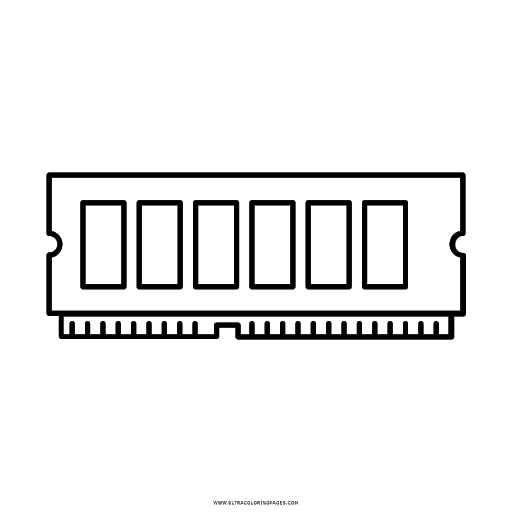
\includegraphics[width=4cm]{memoriaRAM.png}
\centering
\caption{imagen memoria RAM}
\label{fig:memoriaRAM}
\end{figure}

\textbf{Memoria virtual:} Es una parte del disco duro, la cual es previamente reservada para almacenar temporalmente informacíon que ocupa espacio innecesario de la memoria como fragmentos de programas que son menos utilizados. La información allí almacenada está siempre disponible para cuando requiera ser utilizada. 

la memoria virtual, nace como solución al uso excesivo de memoria RAM, cuando se usan simultaneamente programas que ocupan mucho espacio en su ejecución al pasar la información a un 'segundo plano' mientras no se esté usando.
A pesar de ser este un buen recurso, la solución para tener un mejor rendimiento en el equipo, es tener la mayor cantidad de memoria RAM posible y disponible.\\

\textbf{Memoria caché:} Esta memoria se encuentra dentro del microprocesador, y se está dividida en 3 niveles: L1, L2 Y L3. su principal objetivo es hacer que la memoria llegue a su máxima rapidez. Contiene copias de fragmentos de la memoria principal; tiene la información que el microprocesador utiliza de manera más constante, entonces para no tener que recurrir a ellos desde la memoria RAM, se hace una copia en la caché.  
Describiendo su funcionaiento, cuando el procesador trata de leer una palabra de la memoria, comprueba si esta palabra está en la memoria caché. Si lo está, se entrega la palabra al procesador o de lo contrario, un bloque de memoria principal que contiene un cierto número de palabras, se transfiere a la memoria caché y luego la palabra es entegada al procesador.  

la información que más se utiliza, es llevada al primer nivel L1, que funciona a la misma velocidad de los núcleos del microprocesador. Los datos menos utilizados, se encuentran en el segundo nivel L2, que a pesar de que también se encuentra dentro de los nucleos, no es tan rápido como el primer nivel, y el resto de datos se almacenan en el tercer nivel L3. 
 
\subsection{¿Como se gestiona la memoria de un computador?}
%
La forma de gestión de memoria, refiere al almacenamiento temporal de información con la que trabajan los microprocesadores, en donde la procesan y devuelven los resultados pedidos por el usuario.

En principio, el disco duro se encarga de llevar la información hasta una parte de la memoria, para que el microprocesador proceda a realizar las tareas necesarias, y luego la información pasa a otro lugar de la memoria, donde se almacenará ya procesada.
Cuando este ciclo se repita todas las veces necesarias, toda la información previamente procesada, vuelve a ser guardada en el disco duro.

\subsection{¿Que hace que una memoria sea más rápida que otra?}
%
lo que hace que una memoria sea más rapida que otra es la frecuencia y la latencia, ésta ultima es la que mide la cantidad de tiempo que se puede tardar obteniendo la información que se encuentra en cada bit; y la frecuencia por otra parte, es la que mide el rimto de trabajo con el que se comunican los dispositivos encargados de transportar la información.

También hay que tener en cuenta las instrucciones que se encuentran almacenadas en las memorias del computador, ya que de esto depende el tiempo que se tardará en leerlas, ellas viajan a través de un bus de datos, que son circuitos en cobre que reposan sobre la tarjeta o también llamada "placa madre", que es una tarjeta en la cual se conecta estos circutos ya mencionados que conforman el computador.
La velocidad con la que se permite el acceso a la información guardada en cada memoria, depende también de la cantidad de bits o de pulsos eléctricos que se transfieran a través del bus, o sea entre una memoria u otra.
En síntesis, lo que hace que una memoria sea más rápida, es la cantidad de información que se almacene en cada una, y teniendo en cuenta también de su tipo. 

dependiendo de la rapidez de una memoria es el proceso de desarrollo en el funcionamiento de un equipo en general.


\section{Inclusión de imágenes} \label{imagenes}

En la Figura (\ref{fig:memoriaRAM}), se presenta la imagen de una memoria RAM

\bibliographystyle{IEEEtran}
\bibliography{references(taller)}

\end{document}
